\documentclass[12pt, titlepage]{article}
\usepackage[table]{xcolor}
\usepackage{array}
\usepackage{changepage}
\usepackage{graphicx}
\usepackage{lmodern} % for bold teletype
\usepackage{float}
\usepackage[T1]{fontenc}
\usepackage{multirow}
\usepackage{pythonhighlight}
\usepackage{titling}

\newcolumntype{M}[1]{>{\centering\arraybackslash}m{#1}}
\graphicspath{ {./images/} }

% titling
\title{System Design}
\setlength{\droptitle}{-20ex}
\author{Thomas Monson}
\renewcommand\maketitlehookb{\vspace{-3ex}}
\date{}
\renewcommand\maketitlehookd{\vspace{-2ex}}

\definecolor{purple}{HTML}{99479b}
\definecolor{green}{HTML}{00a64f}
\definecolor{blue}{HTML}{00aeef}
\definecolor{red}{HTML}{ed1b23}
\newcommand{\textbt}[1]{\textbf{\texttt{#1}}}

\newcommand{\cols}{
\hline
\multicolumn{1}{|c|}{Name} & \multicolumn{1}{M{1cm}|}{\multirow{2}{*}{\dots}} & Name \\ \cline{1-1} \cline{3-3} 
\multicolumn{1}{|c|}{Value} & \multicolumn{1}{c|}{} & Value \\ \hline
}

\newcommand{\supercolumn}{
\begin{tabular}{|ccc|}
\hline
\multicolumn{3}{|c|}{Super Column Name} \\
\cols
\end{tabular}
}

\newcommand{\columnset}{
\begin{tabular}{|ccc|}
\cols
\end{tabular}
}

\newcommand{\supercolumnset}{
\begin{tabular}{|ccc|c|ccc|}
\hline
\multicolumn{3}{|c|}{Super Column Name} & \multirow{3}{*}{\dots} & \multicolumn{3}{c|}{Super Column Name} \\ \cline{1-3} \cline{5-7}
\multicolumn{1}{|c|}{Name} & \multicolumn{1}{M{1cm}|}{\multirow{2}{*}{\dots}} & Name & & \multicolumn{1}{c|}{Name} & \multicolumn{1}{M{1cm}|}{\multirow{2}{*}{\dots}} & Name \\ \cline{1-1} \cline{3-3} \cline{5-5} \cline{7-7}
\multicolumn{1}{|c|}{Value} & \multicolumn{1}{c|}{} & Value & & \multicolumn{1}{c|}{Value} & \multicolumn{1}{c|}{} & Value \\ \hline
\end{tabular}
}

\setlength\parindent{0pt}

\begin{document}
\maketitle

\tableofcontents
\newpage

\section{System Design Interview Process}

You are given a \textit{problem statement}.

\subsection{Requirements Clarification}

This shows the interview how you deal with ambiguity. It also reduces the scope of the problem to something that can be discussed within the time constraints of an interview.

\subsubsection{Ask Questions}

\begin{itemize}
  \item Users/customers
    \begin{itemize}
      \item Who will use the system?
      \item How will the system be used?
    \end{itemize}
  \item Scale (read/write)
    \begin{itemize}
      \item How many read queries per second?
      \item How many write queries per second?
      \item How much data is queried per request?
      \item Can there be spikes in traffic?
    \end{itemize}
  \item Performance
    \begin{itemize}
      \item What is the expected write-to-read data delay? (batch processing vs. stream processing)
      \item How fast must data be read from the system? (p99 (worst-case) latency) \medskip \\
        \phantom{MM}as fast as possible $\rightarrow$ perform complex operations on write
    \end{itemize}
  \item Cost
    \begin{itemize}
      \item Should the design minimize development cost? (open-source vs. proprietary)
      \item Should the design minimize maintenance cost? (public cloud services vs. on-prem)
    \end{itemize}
\end{itemize}

Requirements clarification gets us closer to defining functional and non-functional requirements.

\subsubsection{Define Functional Requirements}

\textit{Functional requirements} specify system behavior in terms of APIs, a set of operations that the system will support. \\

Write down something that the system must do, convert that into a function, and then generalize as necessary. For example: \\

\begin{adjustwidth}{2em}{0em}

``The system has to \textbf{\textcolor{purple}{count} \textcolor{green}{video} \textcolor{blue}{view} \textcolor{red}{events}}.'' \\

\textbt{\textcolor{purple}{count}\textcolor{blue}{View}\textcolor{red}{Event}(\textcolor{green}{videoId})} \\

\textbt{\textcolor{purple}{count}\textcolor{red}{Event}(\textcolor{green}{videoId}, \textcolor{blue}{eventType})} \\

\textbt{process\textcolor{red}{Event}(\textcolor{green}{videoId}, \textcolor{blue}{eventType}, \textcolor{purple}{functionType})} \\

  \textbt{process\textcolor{red}{Event}s(listOfEvents)} \ (Event is an object here)

\end{adjustwidth}

\subsubsection{Define Non-functional Requirements}

\textit{Non-functional requirements} specify system qualities (e.g. fast, fault-tolerant, secure). \\

Possible non-functional requirements include:
\begin{itemize}
  \item Scalability (ease of increasing capacity to handle load)
  \item Availability (percentage of time that system can be used for production)
  \item Consistency (all nodes have the same view of the data at all times, necessary for correctness)
  \item Performance (requests are serviced quickly)
  \item Durability (data remains persistent, despite catastrophic events)
  \item Reliability (system continues to work, even if parts of it fail)
  \item Maintainability (ease of fixing or upgrading system)
  \item Cost (upfront and over time; hardware, software, and manpower)
\end{itemize}

For example, a video view counting system might have the following requirements:
\begin{itemize}
  \item Scalable: Tens of thousands of video views per second
  \item Performant: A few tens of milliseconds to return total view count for a video
  \item Available: Survives hardware and network failures, no single point of failure
\end{itemize}

\subsection{High-Level Design}

Think about how data gets into the system and how it gets out and draw some components.

\subsection{Detailed Design}

The first thing to understand is what data we need to store, where we should store it, and how we should store it. We need to define a \textit{data model}.

\subsubsection{What to Store}

To count video views, we can store individual events (every click) or we can aggregate data (e.g. per minute) in real-time. \\

\textbf{Individual events:}
\begin{itemize}
  \item Fast writes (get the whole event, push it to the database)
  \item Can slice and dice data as needed
  \item Can recalculate numbers in reports (because we have all the original data)
  \item Slow reads (need to count every event to count views)
  \item Needs a lot of storage, expensive \\
\end{itemize}

\textbf{Aggregated data:}
\begin{itemize}
  \item Fast reads (direct access)
  \item Data is ready for decision making
  \item Can query only the way the data was aggregated (details lost due to aggregation)
  \item Requires data aggregation pipeline
  \item Hard or impossible to fix calculation errors (because we do not have all the original data)
\end{itemize}

If the system must process events within no more than a few minutes after they occur, then we should store individual events (stream processing). If events can be processed hours later, then we can store aggregated data (batch processing). \\

You could also choose both options. For example, store individual events for several days or weeks and then delete them. Also, calculate and store numbers in real-time. This way, you get fast reads, the ability to aggregate data differently, and the ability to fix errors by referencing individual events. The downside to this approach is that the system becomes more complex and expensive.

\subsubsection{Where to Store}

Decide between SQL or NoSQL. \\

Design a distributed system to support your database choice. For SQL, things like partitioning (sharding), replication, proxies (cluster and shard), service registry (Zookeeper).

\subsubsection{How to Store}

If SQL, design database schema. \\
If NoSQL, structure data as it will be queried.

\subsubsection{Processing and Querying Details}

\subsubsection{Technology Stack}

\subsection{Bottlenecks and Tradeoffs}

How to identify bottlenecks: load testing, stress testing, soak testing (Apache JMeter can produce a desired load) \\

Monitoring, metrics, dashboards \\

How to make sure the system is correct: audit systems \\

\section{Components}

\subsection{Domain Name System (DNS) Server}

A \textit{DNS server} is a server that translates hostnames to IP addresses. \\

When a client sends a request to a DNS server for an IP address, it typically caches that IP so it doesn't have to query the DNS server again. If that IP is a server instead of a load balancer, and a client sends all of their requests to that one IP, and those requests are hard, then that server will be overloaded.

\subsection{Content Delivery Network (CDN)}

A \textit{content delivery network} is a geographically distributed network of servers whose purpose is to store data assets (e.g. text, images, video, files, applications) spatially closer to users for high availability and performance.

\subsection{Load Balancer}

\textit{A (hardware or software) component that distributes requests from clients across N servers} \\

Instead of DNS returning the IP of a single server, it can return the IP of the load balancer, which will choose which server to send the request to. This is helpful for \textit{horizontal scaling}. \\

The load balancer can route traffic using various strategies:

\begin{itemize}
  \item \textbf{Random}
  \item \textbf{Least-loaded}
  \item \textbf{Round-robin:} first server 1, then server 2, ..., back to server 1 (by chance, one server could receive the hardest requests and be overloaded)
  \item \textbf{Session/cookies:} send a user to the same server every time (store a hash in a cookie)
  \item \textbf{Layer 4 (Transport):} manage traffic based on network information such as source and destination IP addresses and TCP or UDP ports
  \item \textbf{Layer 7 (Application):} manage traffic based on HTTP/SMTP information like the content of headers, message bodies, and cookies (e.g. send requests for HTML to dedicated HTML server, send requests for images to dedicated image server)
\end{itemize}

If the load balancer sends a client to server 1, and server 1 stores a session for that client, and then the load balancer sends that client to server 2, then server 2 will not have that client's session (problem of \textit{sticky sessions}). This is why it is recommended to store all user-related data (such as sessions) in a centralized data store (\textit{shared storage}). \\

Multiple load balancers are often used for redundancy. They can be configured as active/passive (active dies, passive promotes itself to active by taking over active IP) or active/active. They check on each other by sending heartbeat packets. This configuration results in \textit{high availability} (same concept exists for databases). \\

A Level 7 load balancer is a reverse proxy.

\subsection{Reverse Proxy}

\textit{A web server that acts as an intermediary that forwards client requests to backend servers and forwards server responses to clients} \\

Benefits include:
\begin{itemize}
  \item \textbf{Increased security:} hide information about backend servers, blacklist IPs, limit number of connections per client
  \item \textbf{Increased scalability and flexibility:} clients only see reverse proxy's IP, allowing you to scale servers or change their configuration
  \item \textbf{SSL termination:} decrypt incoming requests or encrypt server responses so backend servers do not have to perform these potentially expensive operations (no need to install X.509 certificates on each server)
  \item \textbf{Compression:} compress server responses
  \item \textbf{Caching:} return a cached response
  \item \textbf{Static content:} serve static content directly (HTML, images, videos)
\end{itemize}

\subsection{Relational Database}

Relational databases traditionally have \textit{ACID transactions} and favor consistency over availability. \\

\begin{itemize}
  \item \textbf{Atomicity:} Each transaction is all or nothing.
  \item \textbf{Consistency:} Any transaction will bring the database from one valid state to another.
  \item \textbf{Isolation:} Executing transactions concurrently has the same results as if the transactions were executed serially.
  \item \textbf{Durability:} Once a transaction has been committed, it will remain so.
\end{itemize}

\subsubsection{Replication}

\textbf{Primary-replica Replication} \medskip

The \textit{primary} serves reads and writes, replicating writes to one or more \textit{replicas}, which serve only reads. Replicas can also replicate to additional replicas in a tree-like fashion. If the primary goes offline, the system can continue to operate in read-only mode until a replica is promoted to a primary or a new primary is provisioned. \\

Additional logic is needed to promote a replica to primary. \\

\textbf{Multi-primary Replication} \medskip

Primaries serve reads and writes and coordinate with each other on writes. If any primary goes down, the system can continue to operate with both reads and writes. \\

A load balancer or additional logic is needed to determine where to write. \\

Most multi-primary systems are either loosely consistent (non-ACID) or have increased write latency due to synchronization. \\

Write conflict resolution is needed more often as more write nodes are added and latency increases. \\

\textbf{Disadvantages}
\begin{itemize}
  \item Data loss, if a primary fails before newly written data can be replicated
  \item Lots of writes $\rightarrow$ replicas may get overloaded $\rightarrow$ unable to serve reads effectively
  \item More replicas $\rightarrow$ more replication $\rightarrow$ more replication lag
  \item More hardware and additional complexity
\end{itemize}

\subsubsection{Federation (Functional Partitioning)}

Federation (or functional partitioning) splits up databases by function. For example, instead of a single, monolithic database, you could have three databases: \textit{forums}, \textit{users}, and \textit{products}. \\

\textbf{Advantages}
\begin{itemize}
  \item Less read and write traffic
  \item Less replication and replication lag
  \item More cache hits (smaller database $\rightarrow$ more of database can fit in memory $\rightarrow$ improved cache locality)
  \item No central primary serializing writes $\rightarrow$ write in parallel with increased throughput \\
\end{itemize}

\textbf{Disadvantages}
\begin{itemize}
  \item Not effective if your schema requires huge functions or tables
  \item Need to update application logic to determine which database to read/write
  \item Joining data from multiple databases is more complex (server link).
  \item More hardware and additional complexity
\end{itemize}

\subsubsection{Sharding}

Sharding splits up databases by data value, such that each database manages only a subset of the data. For example, a users database could be split into shards for last names A--M and N--Z. Sharding by geographic location is also common practice. \\

Sharding is a form of \textit{horizontal partitioning}. \\

\textbf{Advantages}
\begin{itemize}
  \item Less read and write traffic
  \item Less replication and replication lag
  \item More cache hits (smaller database $\rightarrow$ more of database can fit in memory $\rightarrow$ improved cache locality)
  \item Reduced index size (improves performance with faster queries)
  \item If one shard fails, the other shards remain operational (replication needed to avoid data loss).
  \item No central primary serializing writes $\rightarrow$ write in parallel with increased throughput \\
\end{itemize}

\textbf{Disadvantages}
\begin{itemize}
  \item Need to update application logic to work with shards, could result in complex SQL queries
  \item Load may be unbalanced across shards. Rebalancing requires additional complexity. A sharding function based on \textit{consistent hashing} can distribute load more evenly.
  \item Joining data from multiple shards is more complex.
  \item More hardware and additional complexity
\end{itemize}

\subsubsection{Denormalization}

Informally, a \textit{normalized database} is a database that is structured in accordance with a series of so-called \textit{normal forms} in order to reduce data redundancy and improve data consistency. \textit{Denormalization} is the process of storing redundant copies of data in tables in order to avoid expensive joins. Denormalization attempts to improve read performance at the expense of some write performance (in most systems, reads outnumber writes 100:1 or even 1000:1). \\

One example of denormalization is the use of \textit{materialized views} (found in PostgreSQL and Oracle). A materialized view is the cached result of a query. (A materialized view that stores data based on remote tables is called a \textit{snapshot}.) The RDBMS will try to keep redundant data consistent by recomputing the materialized views occasionally. \\

Denormalization can be helpful for federated or sharded databases, as queries across nodes in such systems can be complex. \\

\textbf{Advantages}
\begin{itemize}
  \item Faster reads, especially for partitioned systems
  \item Simpler queries \\
\end{itemize}

\textbf{Disadvantages}
\begin{itemize}
  \item Redundant data
  \item Data may be inconsistent.
  \item Additional complexity required to keep redundant data consistent
  \item Worse than a normalized database when under heavy write load
\end{itemize}

\subsubsection{Query Tuning (SQL Tuning)}

\textit{Query tuning} is the iterative process of improving queries to speed up server performance. It is important to \textit{benchmark} and \textit{profile} the system to simulate and uncover bottlenecks: \\

\textbf{Benchmark:} simulate high-load situations with tools such as \texttt{ab} \medskip \\
\textbf{Profile:} enable tools such as MySQL's \textit{slow query log} to track performance issues \\

Benchmarking and profiling may point you to the following optimizations: \\

\textbf{Tighten up the schema}
\begin{itemize}
  \item 
\end{itemize}

\textbf{Use good indicies}
\begin{itemize}
  \item 
\end{itemize}

\textbf{Avoid expensive joins:} denormalize where performance demands it. \\

\textbf{Partition tables:} break up a table by putting hot spots in a separate table to help keep it in memory. \\

\textbf{Tune the query cache} \\

\subsection{NoSQL Database}

\textit{NoSQL} is an approach to database design that enables the storage and querying of data by some means other than the tabular relations characteristic of relational databases. A NoSQL database may be ``non-SQL" or ``not only SQL". \\

Data is denormalized, and joins are typically done in application code. Most NoSQL stores lack true ACID transactions and favor availability over consistency (opting for eventual consistency). \textit{BASE} is often used to describe the properties of NoSQL databases: \\

\begin{itemize}
  \item \textbf{Basically available:} the system guarantees availability.
  \item \textbf{Soft state:} the state of the system may change over time, even without input.
  \item \textbf{Eventual consistency:} the system will become consistent over a period of time, given that the system does not receive input during that period.
\end{itemize}

\subsubsection{Key-Value Store}

A \textit{key-value store} is essentially a hash map stored in memory or in an SSD. It has $O(1)$ reads and writes. It can maintain keys in lexicographic order, allowing efficient retrieval of key ranges. A value in the store can have metadata stored along with it. \\

Key-value stores are often used for simple data models or for rapidly-changing data, such as an in-memory cache layer. Since they offer only a limited set of operations, complexity is shifted to the application layer if additional operations are needed. \\

A key-value store is the basis for more complex systems, such as a document store or, in some cases, a graph database.

\subsubsection{Document Store}

A \textit{document store} is a key-value store where the values are documents (JSON, XML, binary, etc.). A document stores all the information for a given object. \\

Document stores provide APIs or a query language to query based on the internal structure of the document itself, similar to how many key-value stores provide features to work with a value's metadata. Based on the underlying implementation, documents are organized by collections, tags, metadata, or directories. \\

Document stores provide high flexibility and are often used when working with data that changes occasionally. \\

Implementations: MongoDB, CouchDB, DynamoDB (also a key-value store)

\subsubsection{Wide-Column Store}

The basic unit of data in a \textit{wide-column store} is a \textit{column}, which is a key-value pair where the key is a \textit{column name} and the value is a \textit{column value}: \\

\begin{table}[H]
\centering
\begin{tabular}{|c|}
\hline
Name  \\ \hline
Value \\ \hline
\end{tabular}
\end{table}

Each value contains a timestamp for versioning and conflict resolution. \\

A \textit{super column} is a key-value pair where the key is a \textit{super column name} and the value is a \textit{set of columns}: \\

\begin{table}[H]
\centering
\supercolumn
\end{table}

A \textit{column family} is a collection of key-value pairs where each key is a \textit{row key} and each value is a \textit{set of columns}: \\

\begin{table}[H]
\centering
\begin{tabular}{|c|c|}
\hline
        &            \\
Row Key & \columnset \\
        &            \\
\hline
\end{tabular}
\end{table}

A column family is akin to a table in a relational database. Unlike a relational database, the names and formats of the columns can vary from row to row in the same table. A wide-column store is like a two-dimensional key-value store; given a column family (table), you can access a value with a row key and a column name. \\

A \textit{super column family} is a collection of key-value pairs where each key is a \textit{row key} and each value is a \textit{set of super columns}: \\

\begin{table}[H]
\centering
\begin{tabular}{|c|c|}
\hline
        &                 \\
Row Key & \supercolumnset \\
        &                 \\
\hline
\end{tabular}
\end{table}

A super column family is akin to a \textit{view} on a set of tables in a relational database. \\

Wide-column stores offer high availability and high scalability. They are often used for very large datasets. \\

Implementations: Bigtable (Google), Cassandra (Meta), HBase (open-source)

\subsubsection{Graph Database}

In a graph database, each node is a record and each arc is a relationship between two nodes. Graph databases are optimized to represent complex relationships with many foreign keys or many-to-many relationships. \\

Graphs databases offer high performance for data models with complex relationships, such as a social network.

\subsection{Cache}

A \textit{cache} is a key-value store that acts as a buffer between two layers of a system, often between the application layer and the database layer. It stores data so that future requests for that data can be served faster. \\

Caching improves page load times and can reduce the load on your servers and databases. In this model, the dispatcher (load balancer, reverse proxy) will first lookup if the request has been made before and try to find the previous result in the cache. If it cannot find it, the dispatcher will forward the request to a worker and store the eventual result in the cache. \\

A database often benefits from a uniform distribution of reads and writes across its partitions. Popular items can skew the distribution, causing bottlenecks. Putting a cache in front of a database can help absorb uneven loads and spikes in traffic. \\

\subsubsection{Client Caching}

Caches can be located on the client side (OS or browser). This is the most efficient form of caching because it allows the client to access resources without communicating with a web server. Common files that are cached client-side include images, HTML, stylesheets, and JavaScript libraries.

\subsubsection{CDN Caching}

CDNs are considered a type of cache.

\subsubsection{Web Server Caching}

Reverse proxies (such as Varnish) can serve static and dynamic content directly, by retrieving result from an internal cache. Such proxies are considered \textit{web accelerators} because they reduce website access time. \\

Web servers can also cache requests, returning responses without having to contact application servers.

\subsubsection{Application Server Caching}

In-memory caches (such as Memcached and Redis) are key-value stores between your application and your data storage. Since the data is held in RAM, it is much faster than typical databases where data is stored on disk. RAM is more limited than disk, so cache invalidation algorithms such as \textit{least recently used (LRU)} can help invalidate `cold' entries and keep `hot' data in RAM. \\

Redis has additional features like persistence and built-in data structures such as sorted sets and lists. \\

Generally, you should try to avoid file-based caching, as it makes cloning and auto-scaling more difficult. \\

\textbf{Caching at the query level} \\
Whenever you query the database, hash the query as a key and store the result to the cache. This approach suffers from expiration issues:

\begin{itemize}
  \item Hard to delete a cached result with complex queries
  \item If one piece of data changes such as a table cell, you need to delete all cached queries that might include the changed cell.
\end{itemize}

\textbf{Caching at the object level} \\
See your data as an object, similar to what you do with your application code. Have your application assemble the result from the database into a class instance or a data structure.

\begin{itemize}
  \item Remove the object from cache if its underlying data has changed
  \item Allows for asynchronous processing: workers assemble objects by consuming the latest cached object
\end{itemize}

\subsubsection{Database Caching}

A database usually includes some level of caching in a default configuration, optimized for a generic use case. Tweaking these settings for specific usage patterns can further boost performance.

\subsubsection{Cache-Aside (Lazy Loading) Update Strategy}

The application is responsible for reading and writing from storage. The cache does not interact with storage directly. The application does the following:

\begin{itemize}
  \item Look for entry in cache, resulting in a cache miss
  \item Load entry from the database
  \item Add entry to cache
  \item Return entry
\end{itemize}

\begin{python}
def get_user(self, user_id):
    user = cache.get("user.{0}", user_id)
    if user is None:
        user = db.query("SELECT * FROM users WHERE user_id = {0}", user_id)
        if user is not None:
            key = "user.{0}".format(user_id)
            cache.set(key, json.dumps(user))
    return user
\end{python}

Memcached is generally used in this manner. Only requested data is cached, which avoids filling up the cache with data that isn't requested. \\

\textbf{Disadvantages}
\begin{itemize}
  \item Each cache miss results in three trips.
  \item Data can become stale if it is updated in the database. This issue is mitigated by setting a \textit{time-to-live (TTL)}, which forces a deletion or an update of the cache entry.
  \item When a cache node fails, it is replaced by a new, empty node, increasing latency.
\end{itemize}

\subsubsection{Write-Through Update Strategy}

The application uses the cache as the main data store, reading and writing data to it, while the cache is responsible for reading and writing to the database:

\begin{itemize}
  \item Application adds/updates entry in cache
  \item Cache synchronously writes entry to data store
\end{itemize}

\begin{python}
# Application code
set_user(12345, {"foo":"bar"})
\end{python}

\begin{python}
# Cache code
def set_user(user_id, values):
    user = db.query("UPDATE Users WHERE id = {0}", user_id, values)
    cache.set(user_id, user)
\end{python}

Write-through is a slow overall operation due to the write operation, but subsequent reads of just written data are fast. Users are generally more tolerant of latency when updating data than reading data. Data in the cache is not stale. \\

\textbf{Disadvantages}
\begin{itemize}
  \item When a new node is created due to failure or scaling, it will not cache an entry until that entry is updated in the database. That is, a read request for data not in cache will not put that data in cache. Cache-aside in conjunction with write-through can mitigate this issue.
  \item Most data written may never be read (define a TTL to remove these entries).
\end{itemize}

\subsubsection{Write-Behind (Write-Back) Update Strategy}

In write-behind, the application does the following:

\begin{itemize}
  \item Add/update entry in cache
  \item Asynchronously write entry to the data store, improving write performance (put request in message queue, dequeue request with event processor, write to database)
\end{itemize}

\textbf{Disadvantages}
\begin{itemize}
  \item Data loss if cache fails before its data is written to the database
  \item Harder to implement
\end{itemize}

\subsubsection{Refresh-Ahead Update Strategy}

Configure the cache to automatically refresh any recently accessed cache entry prior to its expiration. \\

Refresh-ahead can result in reduced latency vs read-through if the cache can accurately predict which items are likely to be needed in the future. Not accurately predicting can result in worse performance.

\subsection{Queue (Asynchronism)}

A \textit{message queue} receives, holds, and delivers messages. They facilitate \textit{asynchronous workflows}, which can reduce response time for expensive operations that would otherwise be done in-line. \\

A \textit{task queue} supports scheduling and can be used to run computationally-intensive jobs in the background.

\begin{itemize}
  \item Method 1: do time-consuming work in advance, serve finished work with low request time. For example, complicated web pages can be pre-rendered and stored as static HTML pages on every change.
  \item Method 2: put time-consuming work into a job queue
    \begin{enumerate}
      \item A user starts a computationally intensive task
      \item The frontend sends the task to a job queue and informs the user that the job is being processed
      \item Workers are constantly checking the job queue for jobs. One of them picks up the new job, works on it, and sends a signal to the frontend that the job is done
      \item The frontend is constant checking for ``job is done" signals. It picks up the signal and informs the user that their job is done.
    \end{enumerate}
\end{itemize}

While a job is being processed, a client can optionally do a small amount of work to make it seem like the task has completed. For example, when posting a tweet, the tweet could be instantly posted to your timeline, but it could take some time before your tweet is actually delivered to all of your followers. \\

If queues start to grow significantly, the queue size can become larger than memory, resulting in cache misses, disk reads, and even slower performance. This happens when a producer sends messages to a queue faster than the consumer can process them. A \textit{back pressure} mechanism can help with this by slowing down the producer's rate of sending messages to match the rate at which the consumer can process them. Once the queue gets to a fixed size, clients will get a ``server busy" or HTTP 503 status code. \\

Queues may not be effective for inexpensive operations or real-time workflows. \\

Implementations: RabbitMQ, ActiveMQ, Redis, Amazon SQS, Celery (scheduling)

\section{Concepts}

\subsection{Communication}

\textit{Communication protocols} enable an entity in one host to interact with a corresponding entity at the same layer in another host. At each layer $N$, two entities (layer $N$ peers) exchange \textit{protocol data units} (PDUs) by means of a layer $N$ protocol. Each PDU contains a payload, called the \textit{service data unit} (SDU), along with protocol-related headers or footers. \\

The process of communication between a transmitting device and a receiving device is as follows:

\begin{enumerate}
  \item The data to be transmitted is composed at the topmost layer of the transmitting device (layer $N$) into a PDU.
  \item The layer-$N$ PDU is passed to layer $N-1$, where it is considered an SDU.
  \item At layer $N-1$, the SDU is concatenated with a header and/or footer, producing a layer-$N-1$ PDU. This process is known as \textit{encapsulation}. The PDU is then passed to layer $N-2$.
  \item This process continues until the lowest level is reached, from which the data is transmitted to the receiving device.
  \item At the receiving device, the data is passed from the lowest to the highest layer. Each layer receives the data as a PDU, strips the layer-specific headers/footers from the PDU to produce an SDU, and passes the SDU up a layer, where it will be considered a PDU. At the topmost layer, the data is consumed by an application.
\end{enumerate}

\subsubsection{The OSI Model}

\textbf{Application (Layer 7)} \\

Serves as the window for users and application processes to access the network services. At this layer, a program creates data to be sent or opens data it has received. \\

Facilitates resource sharing, remote file access, remote printer access, directory services, and network management. \\

Protocols include HTTP(S), SMTP, (S)FTP, SSH, DHCP, and DNS. \\

\textbf{Presentation (Layer 6)} \\

Formats the data to be presented to the Application layer. It can be viewed as the "Translator" for the network. Sometimes called the "syntax layer" because it relieves application-layer protocols of concern regarding syntactical differences in data representation within end-user systems. \\

Facilitates character code translation, data conversion, data compression, data encryption, and character set translation. \\

Protocols include TLS and SSL. Works with standards like JPEG, ASCII, and EBCDIC. \\

\textbf{Session (Layer 5)} \\

Allows session establishment between processes running on different stations. \\

Facilitates session establishment (log-on), maintenance, and termination (log-off), and session support (security, name recognition, logging). \\

The RPC protocol is executed at this layer. \textit{Logical ports} operate at this layer. \\

\textbf{Transport (Layer 4)} \\

Ensures that messages are delivered error-free, in sequence, and with no losses or duplications. \\

Facilitates message segmentation, message acknowledgement, message traffic control, and session multiplexing. \\

Protocols include TCP and UDP. \\

\textbf{Network (Layer 3)} \\

Controls the operations of the subnet, deciding which physical path the data takes. Transfers \textit{packets} from one node to another in a different network. \\

Facilitates routing, subnet traffic control, frame fragmentation, logical-physical address mapping, and subnet usage accounting. \\

Protocols include IP, IPX, and ICMP. Routers operate at this layer. \\

\textbf{Data Link (Layer 2)} \\

Provides error-free transfer of \textit{data frames} from one node to another over the Physical layer. \\

Facilitates the establishment and termination of the logical link between nodes, frame traffic control, frame sequencing, frame acknowledgement, frame delimiting, frame error checking, and media access control. \\

Protocols include PPP, Ethernet, and Wi-Fi. \textit{Switches}, \textit{bridges}, and \textit{wireless access points} (WAPs) operate at this layer. \\

\textbf{Physical (Layer 1)} \\

Concerned with the transmission and reception of the unstructured raw bit stream over the physical medium. \\

Facilitates data encoding, physical medium attachment, transmission technique (baseband or broadband), and physical medium transmission (bits and volts). \\

Cables and hubs operate at this layer. \\

\subsubsection{Hypertext Transfer Protocol (HTTP)}

HTTP is an application layer request/response protocol for encoding and transporting data between a client and a server.

\begin{table}
  \begin{center}
    \begin{tabular}{|l|l|c|c|l|}
      \hline
      \textbf{Method} & \textbf{Description} & \textbf{Idempotent} & \textbf{Safe} & \textbf{Cacheable} \\ \hline
      GET & & Yes & Yes & \\ \hline
      POST & & No & No & \\ \hline
      PUT & & Yes & No & \\ \hline
      PATCH & & No & No & \\ \hline
      DELETE & & Yes & No & \\ \hline
      CONNECT & & & & \\ \hline
      TRACE & & & & \\ \hline
      OPTIONS & & & & \\ \hline
      HEAD & & & & \\ \hline
    \end{tabular}
  \end{center}
\end{table}

An HTTP message consists of:
\begin{itemize}
  \item A \textit{start-line} (either a \textit{request-line} or a \textit{status-line}, depending on whether the message is a request or a response)
  \item Zero or more \textit{header field lines}, also known as \textit{headers}, which are key-value pairs, each followed by a \texttt{CR-LF} character sequence
  \item An empty line (i.e. a line with nothing preceding the \texttt{CR-LF}), indicating the end of the header fields
  \item Optionally, a message body (payload) \\
\end{itemize}

An HTTP request-line is a space-separated sequence of the following:
\begin{itemize}
  \item An HTTP method (e.g. \texttt{GET}, \texttt{POST}, etc.)
  \item A \textit{request-target} (identifies the resource upon which to apply the request) \\\\
  Can be in any of the following formats, depending on the method used:
    \begin{itemize}
      \item \textit{origin form}, an absolute path. This is the most common form, used when requests are made to an origin server. \medskip \\
        \phantom{MM}\texttt{/pub/WWW/ThePage.html} (cannot be empty, \texttt{/} at least)
      \item \textit{absolute form}, a complete URL. Mostly used when a \texttt{GET} request is made to a proxy. \medskip \\
        \phantom{MM}\texttt{https://www.website.com/pub/WWW/ThePage.html}
      \item \textit{authority form}, a domain name and port. Only used with \texttt{CONNECT} when setting up an HTTP tunnel. \medskip \\
        \phantom{MM}\texttt{website.com:80}
      \item \textit{asterisk form}, \texttt{*} (not a resource, but the server itself). Used with \texttt{OPTIONS}.
    \end{itemize}
  \item An HTTP version (e.g. \texttt{HTTP/1.1})
  \item \texttt{CR-LF}
\end{itemize}

For example, a request-line could look like:
\begin{center}
\texttt{GET https://www.website.com/pub/WWW/ThePage.html HTTP/1.1}
\end{center}

An HTTP status-line is a space-separated sequence of the following:
\begin{itemize}
  \item An HTTP version
  \item A \textit{status-code} (3-digit integer code describing the server's attempt to serve the client's request)
  \item A \textit{reason-phrase} (a human readable description of the status-code)
\end{itemize}

For example, a status-line could look like: \texttt{HTTP/1.1 200 OK} \\

There are three types of HTTP headers:
\begin{itemize}
  \item \textit{Request header}: contains information about the resource to be accessed or about the client itself
  \item \textit{Response header}: contains information about the response or about the server itself
  \item \textit{Representation header}: contains metadata about the resource in the message body
\end{itemize}

Some important headers include:
\begin{itemize}
  \item \texttt{Host}
  \item \texttt{Accept}
  \item \texttt{Authorization}
  \item \texttt{User-Agent}
  \item \texttt{Content-Type}
  \item \texttt{Content-Length}
  \item \texttt{Cookie}
  \item \texttt{Set-Cookie}
  \item \texttt{Server}
\end{itemize}

\subsubsection{Transmission Control Protocol (TCP)}

TCP is a connection-oriented protocol over an IP network. That is, a sender and receiver must first establish a connection based on agreed parameters, and they do this through a \textit{three-way handshake}:
\begin{enumerate}
  \item Alice sends Bob a synchronize message (SYN) with sequence number $x$
  \item Bob sends Alice a synchronize-acknowledgement message (SYN-ACK) with sequence number $y$ and acknowledgement number $x+1$
  \item Alice sends Bob an acknowledgement message (ACK) with acknowledgement number $y+1$
\end{enumerate}

All packets sent are guaranteed to reach the destination in the original order and without corruption by means of:
\begin{itemize}
  \item Sequence numbers and checksum fields for each packet
  \item Acknowledgement packets and automatic retransmission
\end{itemize}

If the sender does not receive a correct response, it will resend the packets. If there are multiple timeouts, the connection is dropped. TCP also implements \textit{flow control} and \textit{congestion control}. These guarantees cause delays and generally result in less efficient transmission than UDP. \\

To ensure high throughput, web servers can keep a large number of TCP connections open, resulting in high memory usage. Connection pooling can help with this, in addition to switching to UDP where applicable. \\

TCP is useful for applications that require high reliability but are less time critical. Some examples include web servers, database info, SMTP, FTP, and SSH. \\

Use TCP over UDP when:
\begin{itemize}
  \item You need all of the data to arrive intact.
  \item You want to automatically make a best estimate use of the network throughput.
\end{itemize}

Some TCP ports:
\begin{itemize}
  \item 80: HTTP requests (can be used once an encrypted request from the Internet is past the firewall of a system)
  \item 443: HTTPS requests
  \item 22: SSH requests
  \item 3306: MySQL requests
\end{itemize}

\subsubsection{User Datagram Protocol (UDP)}

UDP is connectionless. Datagrams (analogous to packets) are guaranteed only at the datagram level. Datagrams might reach their destination out of order or not at all. UDP does not support congestion control. Without the guarantees that TCP support, UDP is generally more efficient. \\

UDP is less reliable but works well in real-time use cases such as VoIP, video chat, streaming, and real-time multiplayer games.

Use UDP over TCP when:
\begin{itemize}
  \item You need the lowest latency.
  \item Late data is worse than loss of data.
  \item You want to implement your own error correction.
\end{itemize}

\subsubsection{Remote Procedure Call (RPC)}

An RPC is a kind of function call that, when made by a client, causes a procedure to be executed in a different address space, typically on a remote server. The call is written in code just as a local procedure call would be. That is, the programmer does not need to write out the details for remote interaction explicitly. RPCs are usually slower and less reliable than local calls, so it is helpful to distinguish them. \\

An RPC is made by means of a request/response protocol:
\begin{itemize}
  \item The client program calls a (local) client stub procedure. Parameters (procedure ID and arguments) are pushed onto the stack.
  \item The client stub procedure marshals the parameters into a request message.
  \item The client communication module sends the message from the client to the server.
  \item The server communication module passes the incoming packets to the server stub procedure.
  \item The server stub procedure unmarshals the parameters from the message, passes the arguments to the server procedure matching the procedure ID, and calls that procedure.
  \item The server sends its response by repeating the steps above in the other direction.
\end{itemize}

RPCs expose behaviors. REST tends to be used more often for public APIs. \\

RPC frameworks include Protobuf, Thrift, and Avro. \\

\textbf{Disadvantages}
\begin{itemize}
  \item RPC clients become tightly coupled to the service implementation.
  \item A new API must be defined for every new operation or use case.
  \item It can be difficult to debug RPCs.
\end{itemize}

\subsubsection{Representational State Transfer (REST)}

REST is a \textit{software architectural style} that describes how a very large, distributed network of computers that share resources amongst each other---like the Internet---should behave. Because REST was designed with a global-scale system in mind, it specifies that the coupling between client and server should be as loose as possible, to facilitate large-scale adoption. \\

Representation state transfer means that a server will respond with a \textit{representation of a resource} (often an HTML, JSON, or XML document), and that representation will contain hyperlinks that can be followed to make the state of the system change. A client only needs to know the identifier of the first resource it requests; all other identifiers will be discovered in responses. \\

The six architectural constraints of REST APIs:
\begin{itemize}
  \item \textbf{Client/server:} Clients should be separated from servers by a well-defined interface. UI logic should not be coupled with business logic and data-storage logic.
  \item \textbf{Stateless:} When a client makes a request, it should include all of the information necessary for the server to fulfill the request. The server should never have to rely on information from previous requests from the client. If any such information is important, then the client should send it as part of the current request.
  \item \textbf{Cacheable:} Responses should indicate whether or not their data can be cached and for how long. If data is cacheable, the client should automatically cache it and retrieve the data from the cache instead of making an HTTP request for the same information. This reduces unnecessary client-server interaction and improves the availability of servers.
  \item \textbf{Uniform interface:} There should be a standard and uniform way of interacting with servers. Querying resources should allow the client to request other actions and resources without knowing about them in advance.
  \begin{enumerate}
    \item \textbf{Identification of resources:} Resources should be identified by a unique and stable indentifier. Use the URI standard to identify resources.
    \item \textbf{Manipulation of resources through representations:} Clients should get a uniform representation of a resource that contains enough information to update or delete that resource. Use the HTTP standard to describe communication.
    \item \textbf{Self-descriptive messages:} Messages sent between the client and server should contain all of information that the receiver needs to process the message successfully. That is, messages contain not only representations of data but metadata describing the payload as well. Use IANA media types (MIME types) to identify the format of representations and use RDF vocabulary to describe metadata.
    \item \textbf{Hypermedia As The Engine Of Application State (HATEOAS):} A representation of a resource that is sent to a client should have enough information, in the form of hyperlinks, to allow that client to dynamically discover other resources and drive other interactions. This allows a client to "browse" an API similar to how one would browse a webpage. Also, a client will not need to hardcode API URLs in its codebase; instead, they can simply reference a property in the representation they have received whose value is a hyperlink.
  \end{enumerate}
  \item \textbf{Layered system:} A client should not be able to tell whether it is connected directly to an end server or to an intermediary along the way. In other words, there shouldn't be a functional difference between interacting with a single server or a layered system.
  \item \textbf{Code-On-Demand (optional):} A server should be able to send executable code to a client to extend the functionality of that client.
\end{itemize}

REST APIs expose data. Because it is stateless, REST is great for horizontal scaling and partitioning. \\

\textbf{Disadvantages}
\begin{itemize}
  \item Because REST is focused on exposing data, it might not be a good fit if resources are not naturally organized or accessed in a simple hierarchy. For example, returning all updated records from the past hour matching a particular set of events is not easily expressed as a path. With REST, it is likely to be implemented with a combination of URI path, query parameters, and possibly a request body.
  \item REST relies on HTTP methods, which may not be able to describe a use case well. For example, moving expired documents to the archive folder may not be able to be expressed with a single HTTP request.
  \item Fetching complicated resources with nested hierarchies requires multiple round-trips between the client and server to render single views (e.g. fetching content of a blog entry and the comments on that entry). For mobile applications operating in variable network conditions, these multiple round-trips are highly undesirable.
  \item Over time, more fields might be added to an API response, and older clients will receive all new data fields, even those that they do not need. As a result, payload size and latency increases.
\end{itemize}

\subsubsection{GraphQL}

\subsubsection{WebSocket}

\subsubsection{Simple Object Access Protocol (SOAP)}

\subsection{Application Layer}

You can separate your servers into \textit{web servers} (serve static content) and \textit{application servers} (serve dynamic content by means of business logic), and you can scale each layer independently. For example, you could add applicaition servers to support a new API without necessarily adding web servers. \\

\textit{Microservices} are independently deployable, small, modular services. Each service runs a unique process and communicates through a well-defined, lightweight mechanism to serve a business goal. \\

Systems such as Consul, Etcd, and Zookeeper can help services find each other by keeping track of registered names, addresses, and ports.

\subsection{Scalability}

\begin{itemize}
  \item \textit{Vertical scaling}: building up computational resources of a single machine
  \item \textit{Horizontal scaling}: acquiring more machines to serve your application
  \item Every server should contain exactly the same codebase and should not store any user-related data, like sessions or profile pictures, on local disc or memory.
  \item Sessions should be stored in a centralized data store which is accessible to all your application servers. It can be an external database or an external persistent cache, like Redis.
  \item You can create an \textit{image file} from one of your application servers and use it to clone another server instance.
\end{itemize}

\subsection{CAP Theorem}

\textit{Would you prefer to show stale data or no data?} \\

Any distributed data store can provide only two of the following three guarantees:
\begin{itemize}
  \item Consistency: every read receives the most recent write or an error
  \item Availability: every request receives a (non-error) response, without guarantee that it contains the most recent write
  \item Partition tolerance: the system continues to operate despite an arbitrary number of messages being dropped (or delayed) between nodes (network failure)
\end{itemize}

You need to support partition tolerance because networks are not reliable. So you must choose between consistency and availability.

\begin{itemize}
  \item CP: waiting for a response from the partitioned node might result in a timeout error. Good if business needs atomic reads and writes.
  \item AP: responses return the most readily available version of the data, which might not be the latest. Writes might take some time to propagate when the partition is resolved. Good when system needs to continue working despite external errors (eventual consistency).
\end{itemize}

Consistency patterns:
\begin{itemize}
  \item Weak consistency: after a write, reads may or may not see it.
  \item Eventual consistency: after a write, reads will eventually see it.
  \item Strong consistency: after a write, reads will see it.
\end{itemize}

\subsection{RAID (Redundant Array of Independent Disks)}

\begin{itemize}
  \item RAID0 (\textit{striping}): two drives, write data in "stripes", effectively double read/write speeds
  \item RAID1 (\textit{mirroring}): two drives, mirror data between them for redundancy
  \item RAID5 (\textit{distributed parity}): $N$ drives, system can operate with $N - 1$ drives without data loss (one failure allowed), parity information is distributed across drives
  \item RAID6 (\textit{dual parity}): RAID5 + another drive, two parity blocks per stripe, two failures allowed
  \item RAID10 (\textit{striping of mirrors}): four drives, RAID0 + RAID1
\end{itemize}

\section{To Do}

\begin{itemize}
  \item GraphQL (can fetch multiple resources with a single request (query) without fetching data that is not needed)
  \item gRPC
  \item WebSocket (supports bidirectional communication (not request/response, client and server can exchange messages in any order))
  \item Storage Engines
  \item Object Storage
  \item Dead-letter queue
  \item API gateway
  \item Blocking vs. non-blocking IO
  \item Gossip protocol
  \item Service discovery (client-side and server-side), service registry (Zookeeper)
\end{itemize}

\appendix
\newpage

\section{Database Markup Language (DBML)}

This is a domain-specific language (DSL) for defining database schemas.

\begin{verbatim}
Table users {
    id integer
    username varchar
    role varchar
    created_at timestamp
}

Table posts {
    id integer [pk]
    title varchar
    body text [note: 'Content of the post']
    user_id integer [ref: > users.id] // foreign key
    created_at timestamp
}
\end{verbatim}

A \textit{primary key} is an attribute (column) that uniquely specifies a tuple (row) in a relation (table). It can also be a \textit{minimal superkey} (\textit{candidate key}), a minimal set of attributes that together uniquely specify a tuple. \\

A \textit{foreign key} is an attribute or set of attributes that references the primary key of another table. The foreign key should be equal to the primary key in some row of the primary table (\textit{referential integrity constraint}). \\

There are four types of relationships:
\begin{itemize}
  \item One-to-one: \texttt{users.id - user\_infos.user\_id}
  \item One-to-many: \texttt{users.id < posts.user\_id}
  \item Many-to-one: \texttt{posts.user\_id > users.id}
  \item Many-to-many: \texttt{authors.id <> books.id}
\end{itemize}

\section{Glossary}

\textit{hypertext}: electronic text with references (hyperlinks) to other electronic text that the reader can immediately access. It is "hyper" in the sense that it goes "beyond" the linear constraint of written text.

\newpage
\section{Quicksheet}

Load Balancer \\
Reverse Proxy \\
API Gateway \\

\newpage
\pagenumbering{gobble} % turn off page numbering

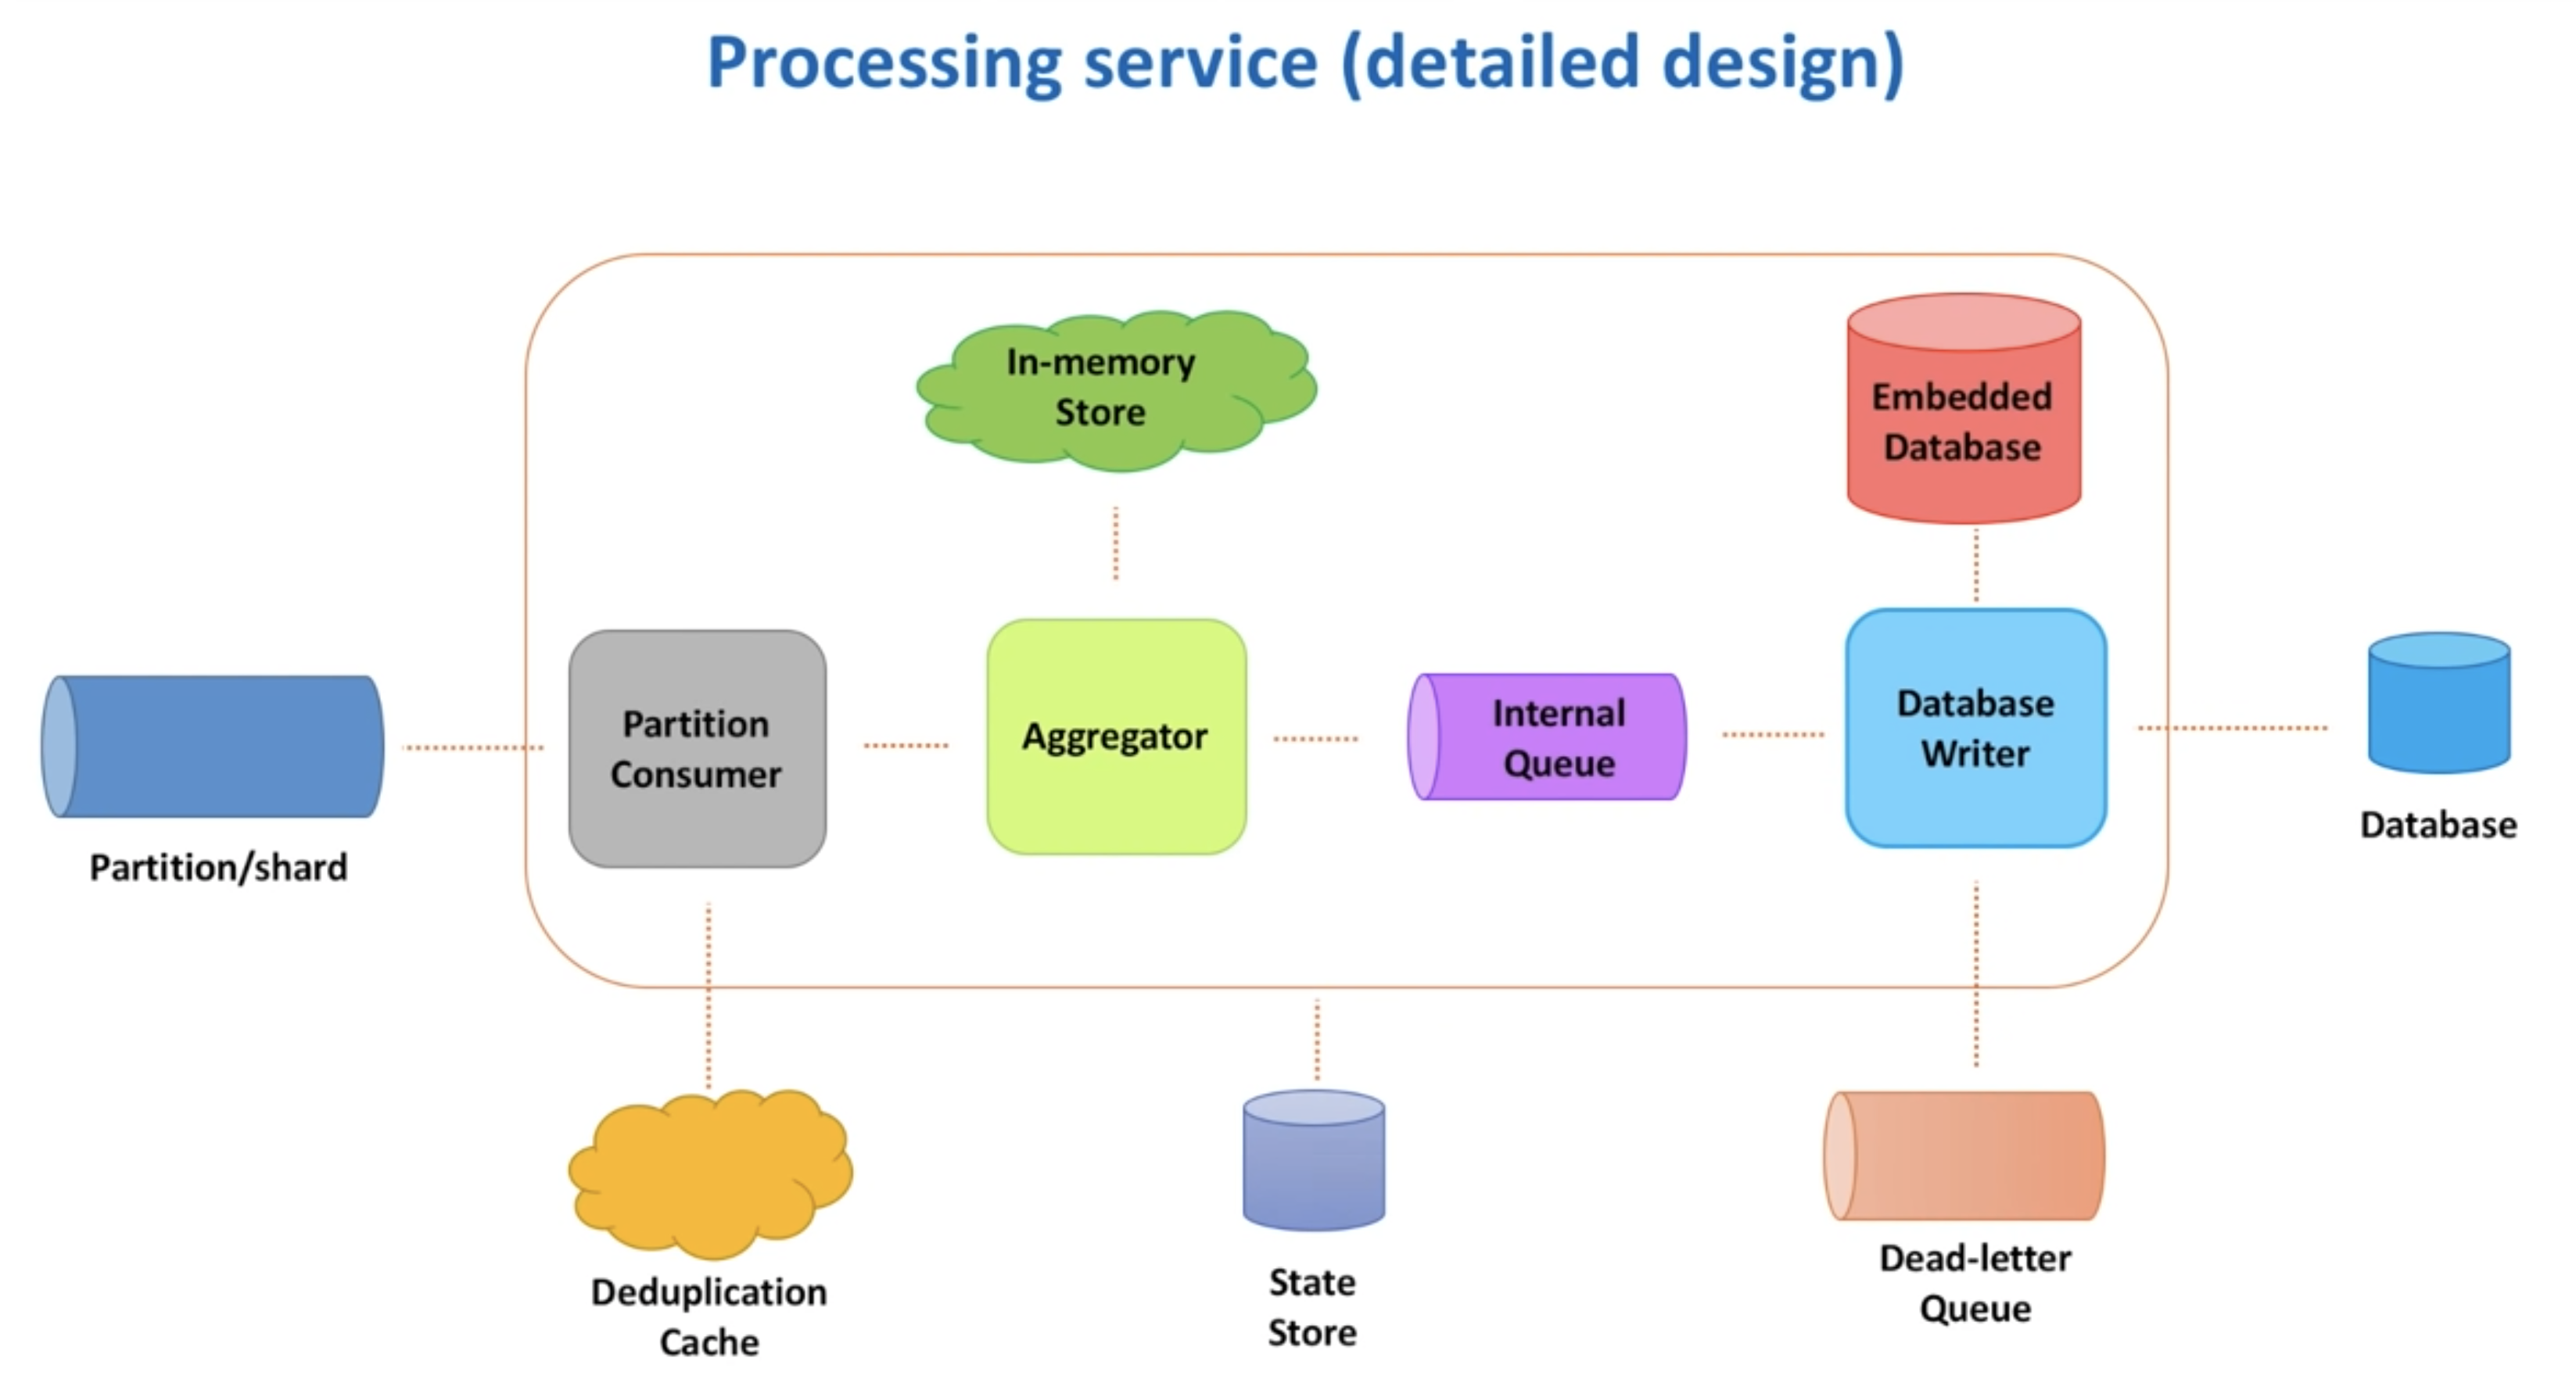
\includegraphics[scale=0.35, angle=90]{processing-service}
\newpage
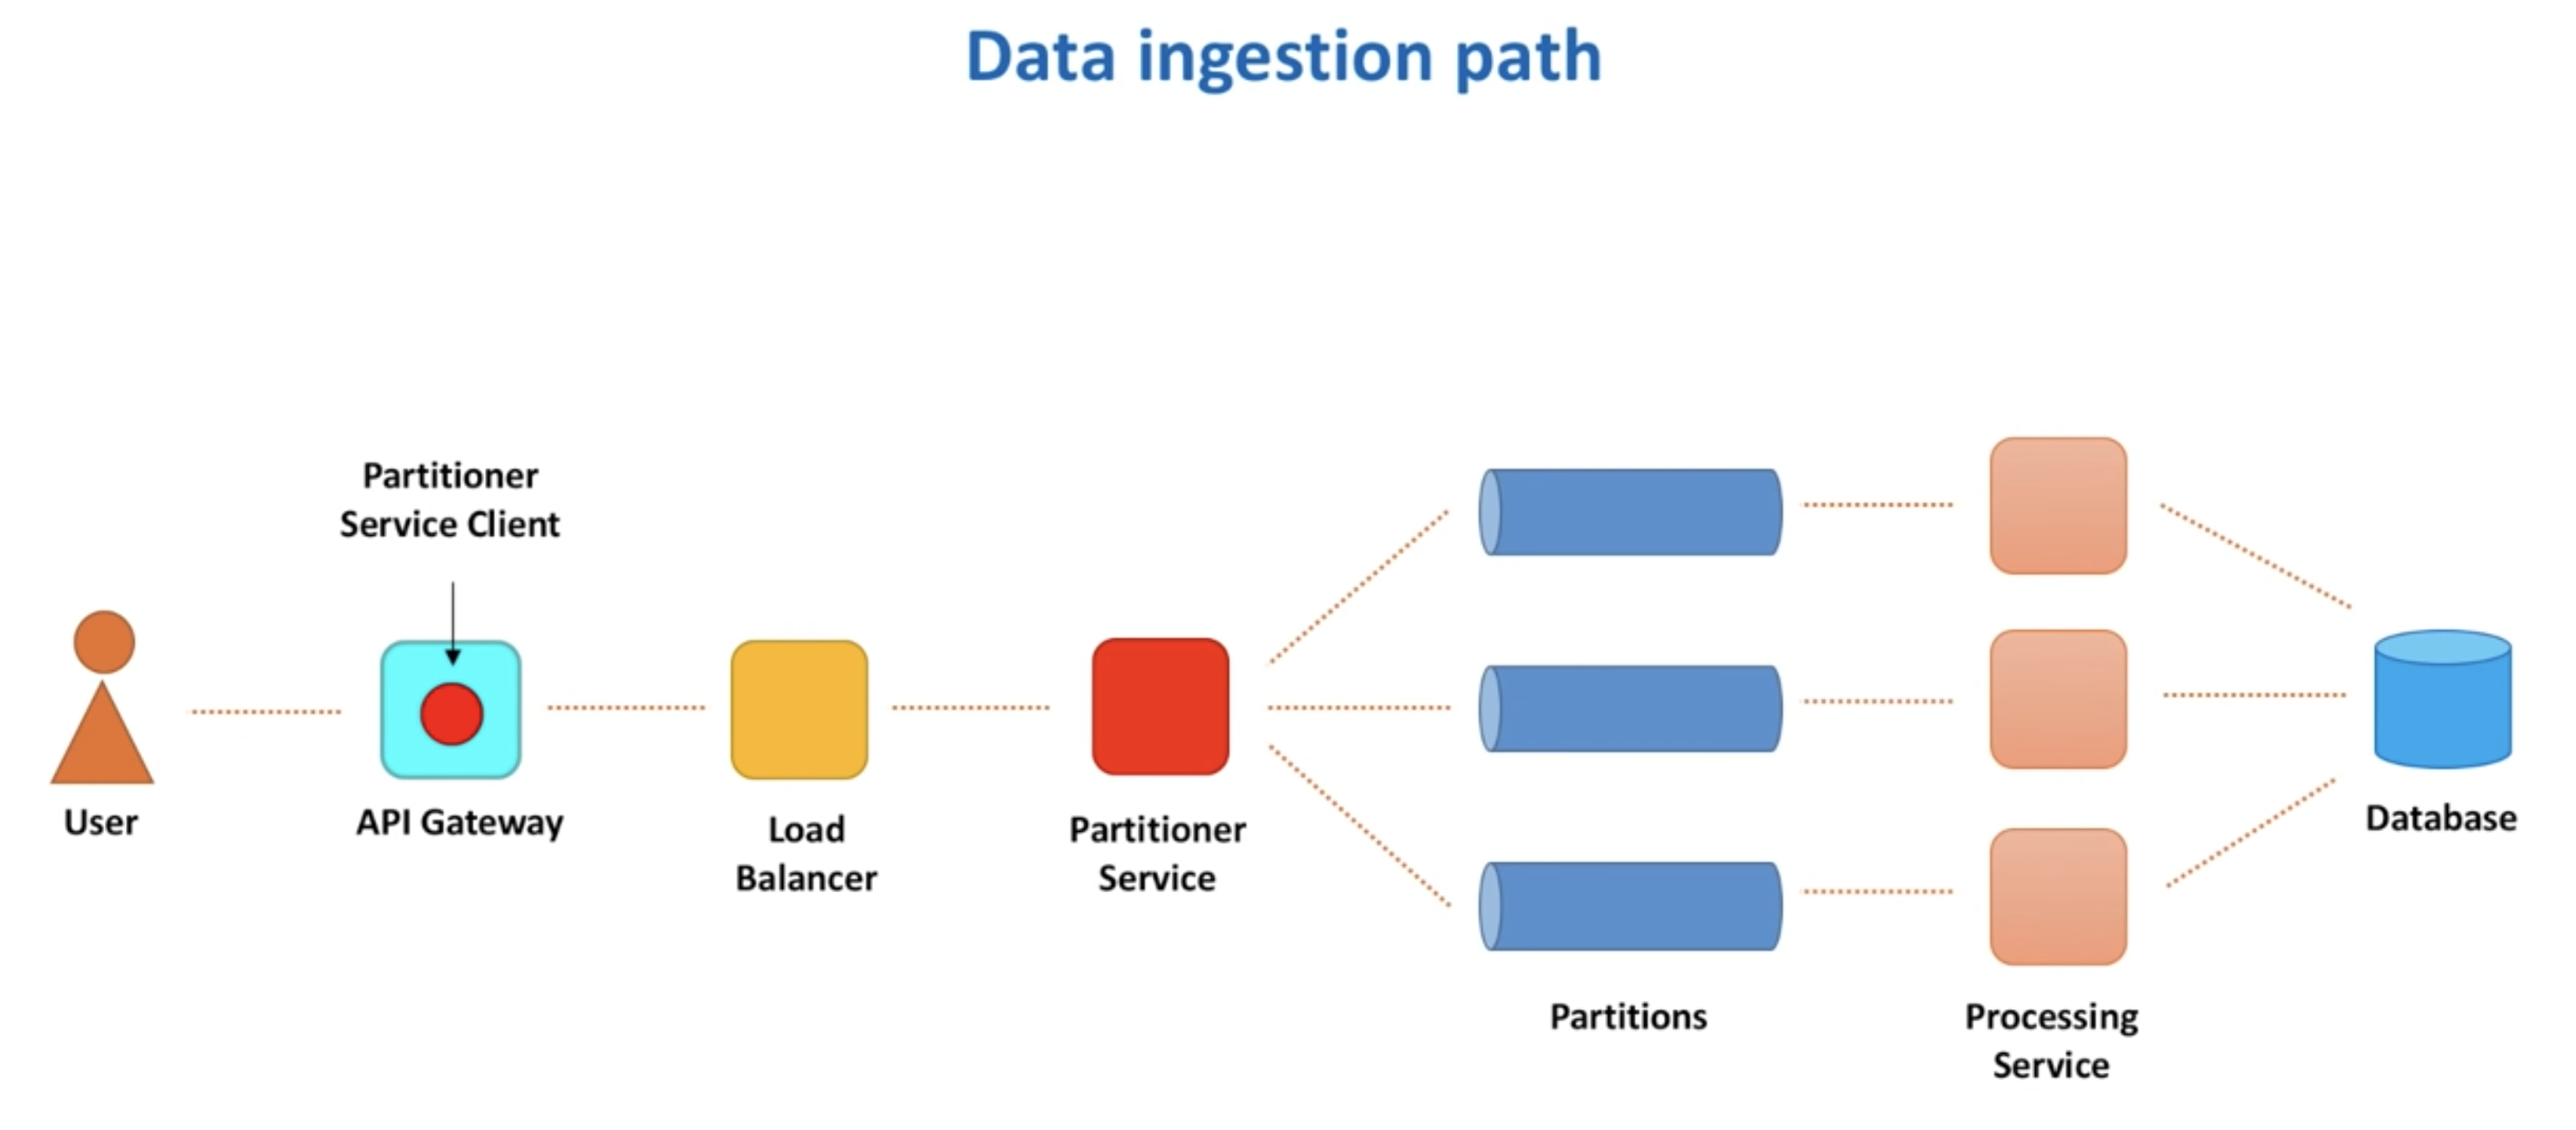
\includegraphics[scale=0.35, angle=90]{data-ingestion}
\newpage
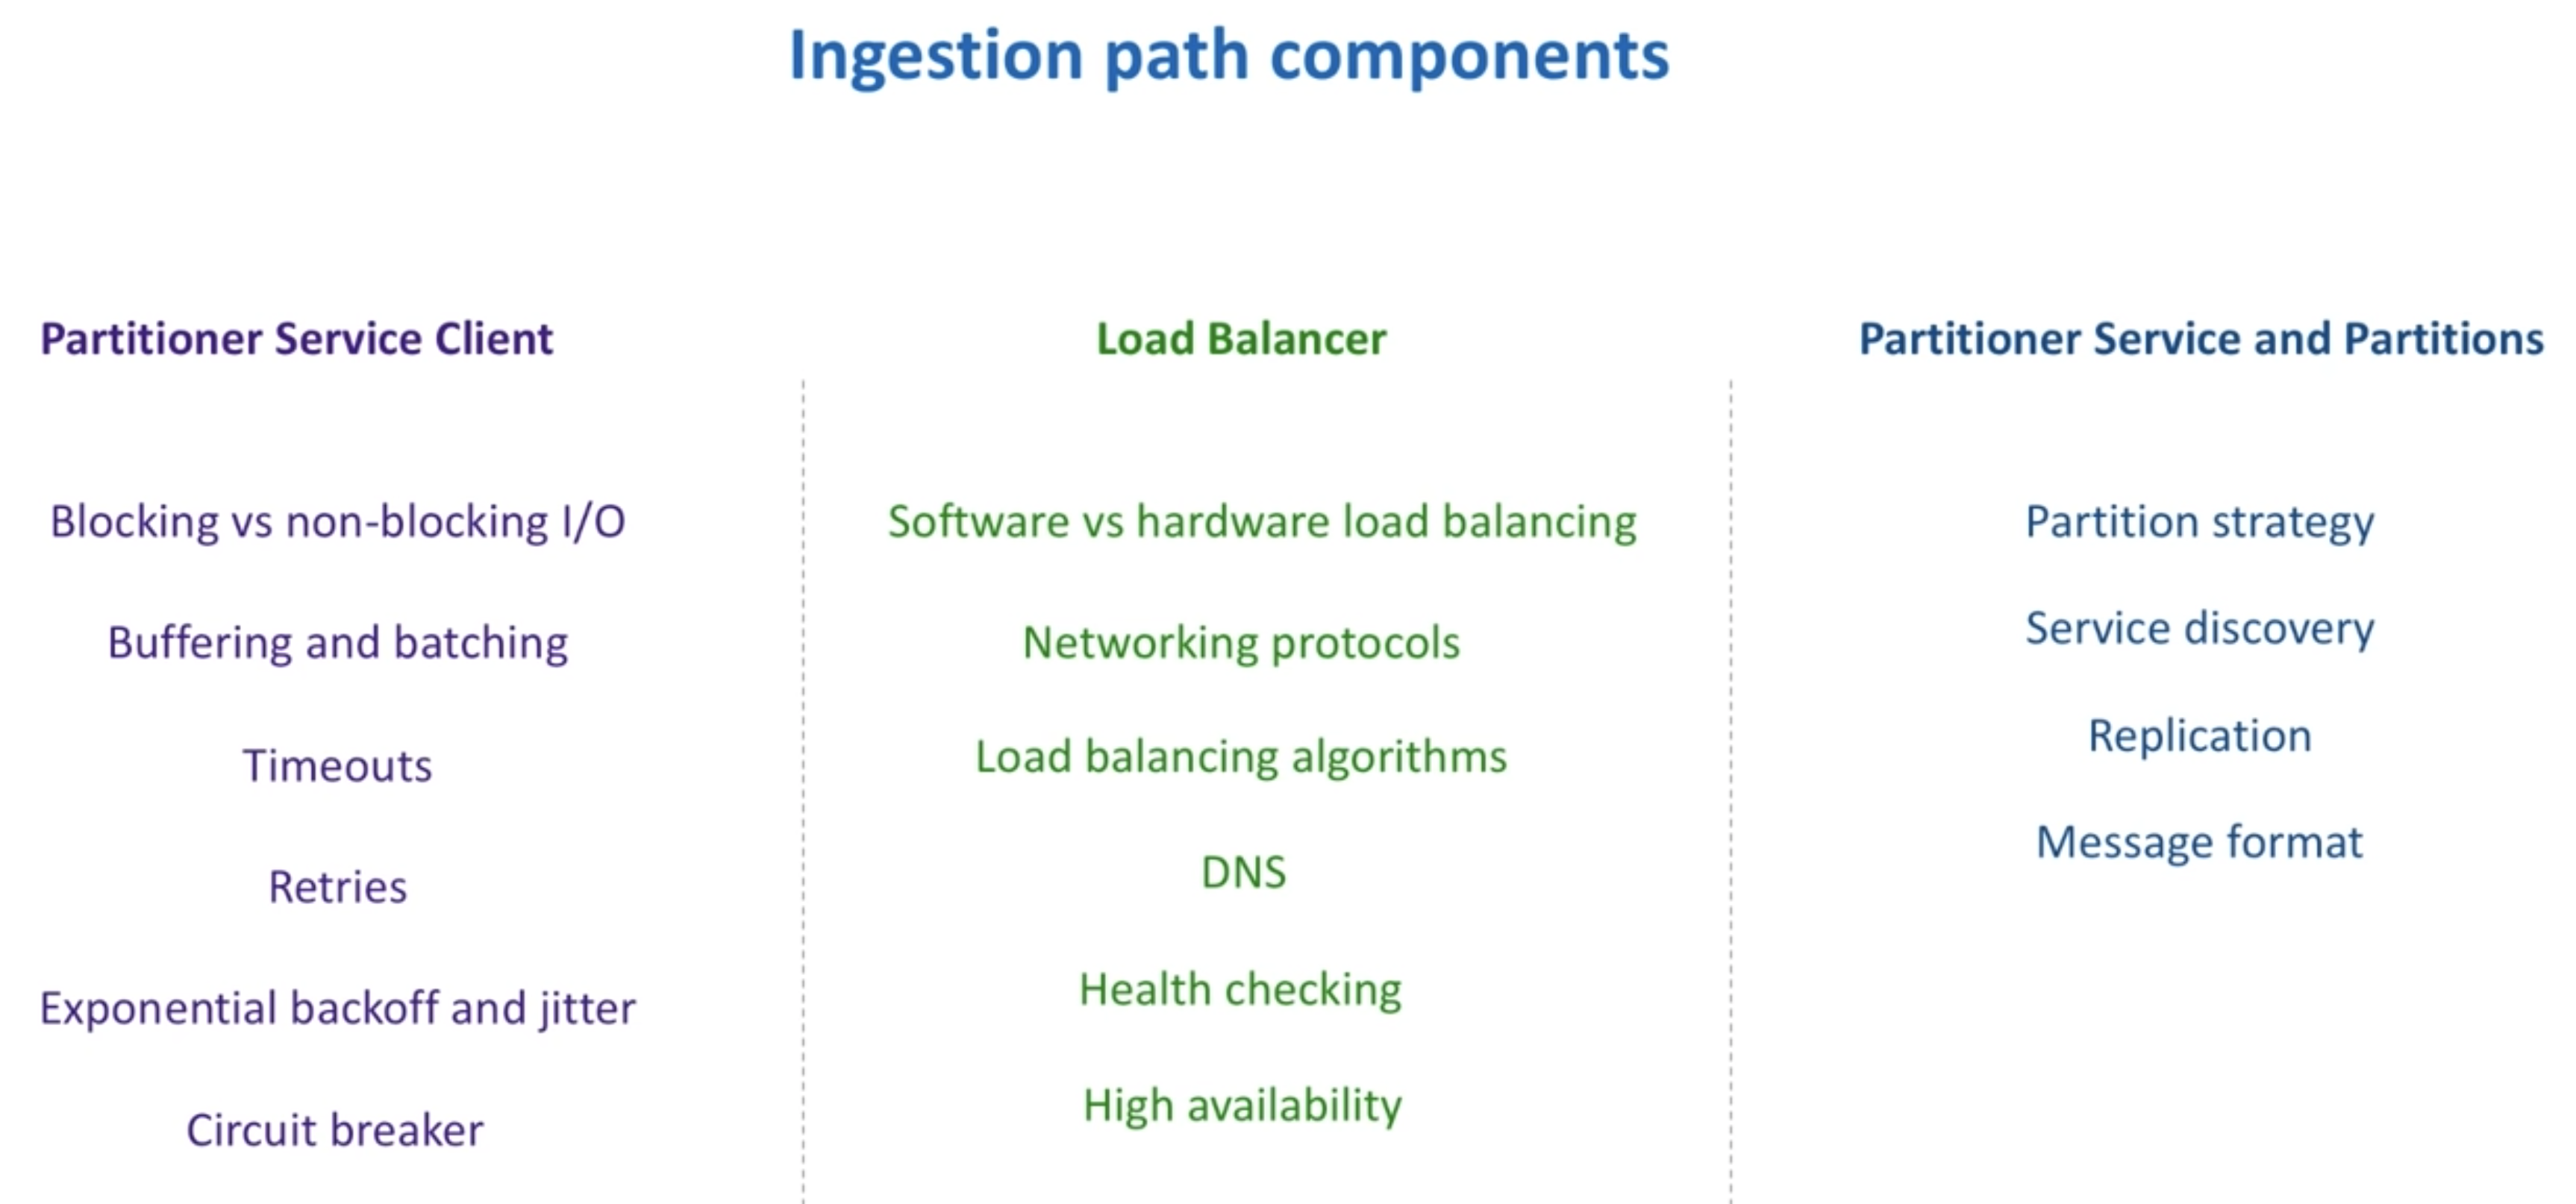
\includegraphics[scale=0.35, angle=90]{data-ingestion-details}
\newpage
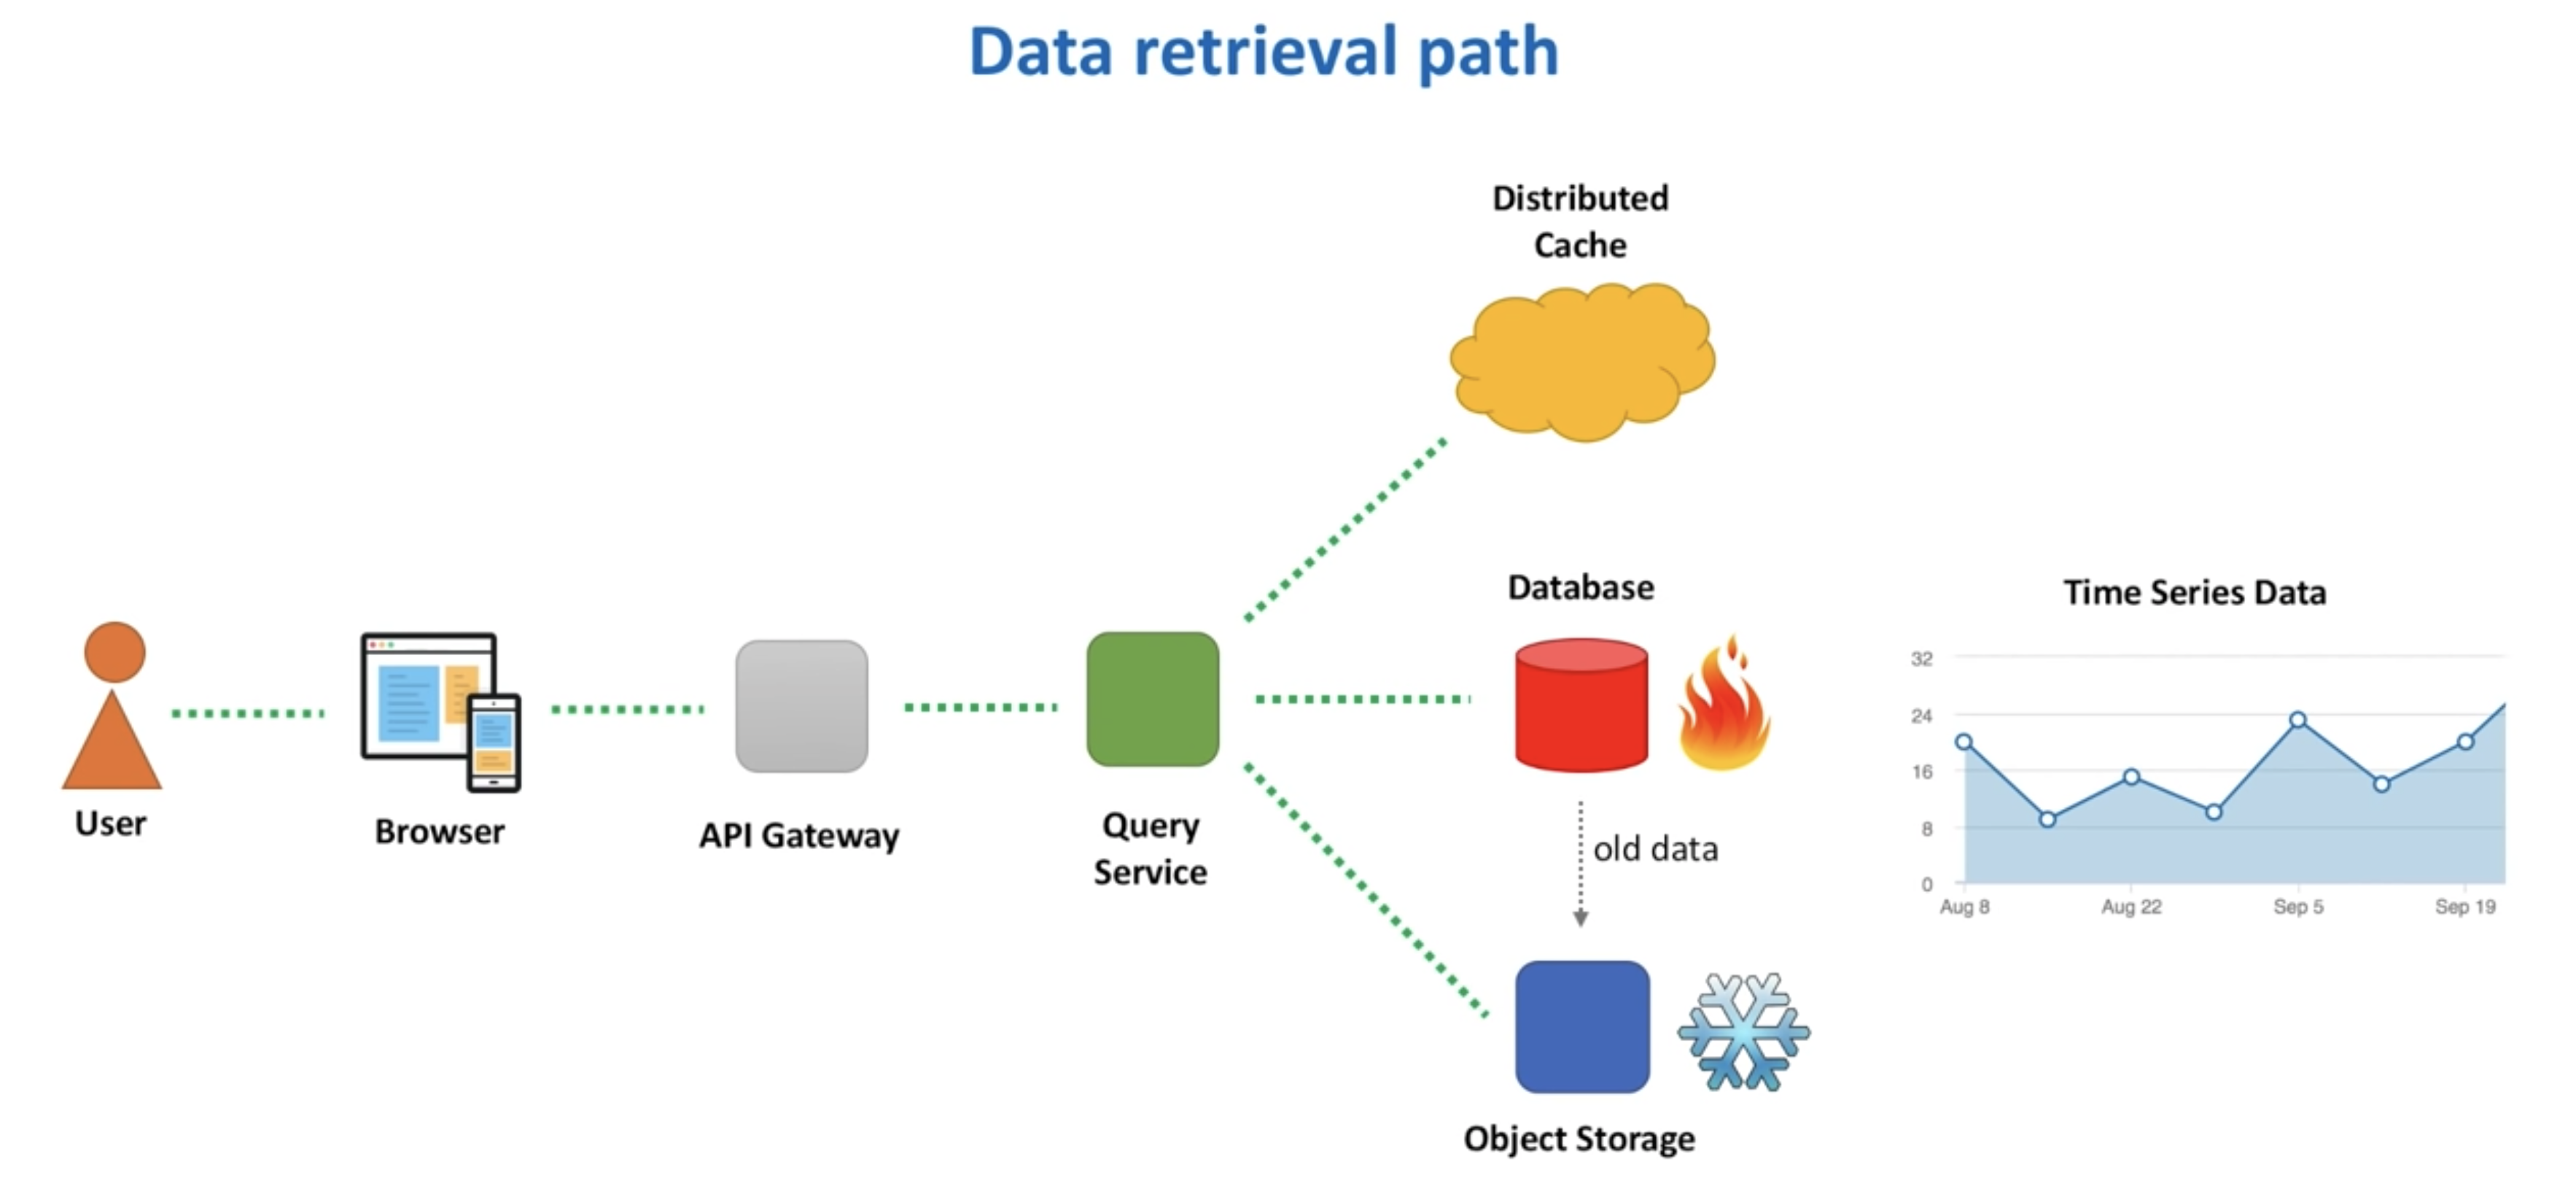
\includegraphics[scale=0.35, angle=90]{data-retrieval}
\newpage
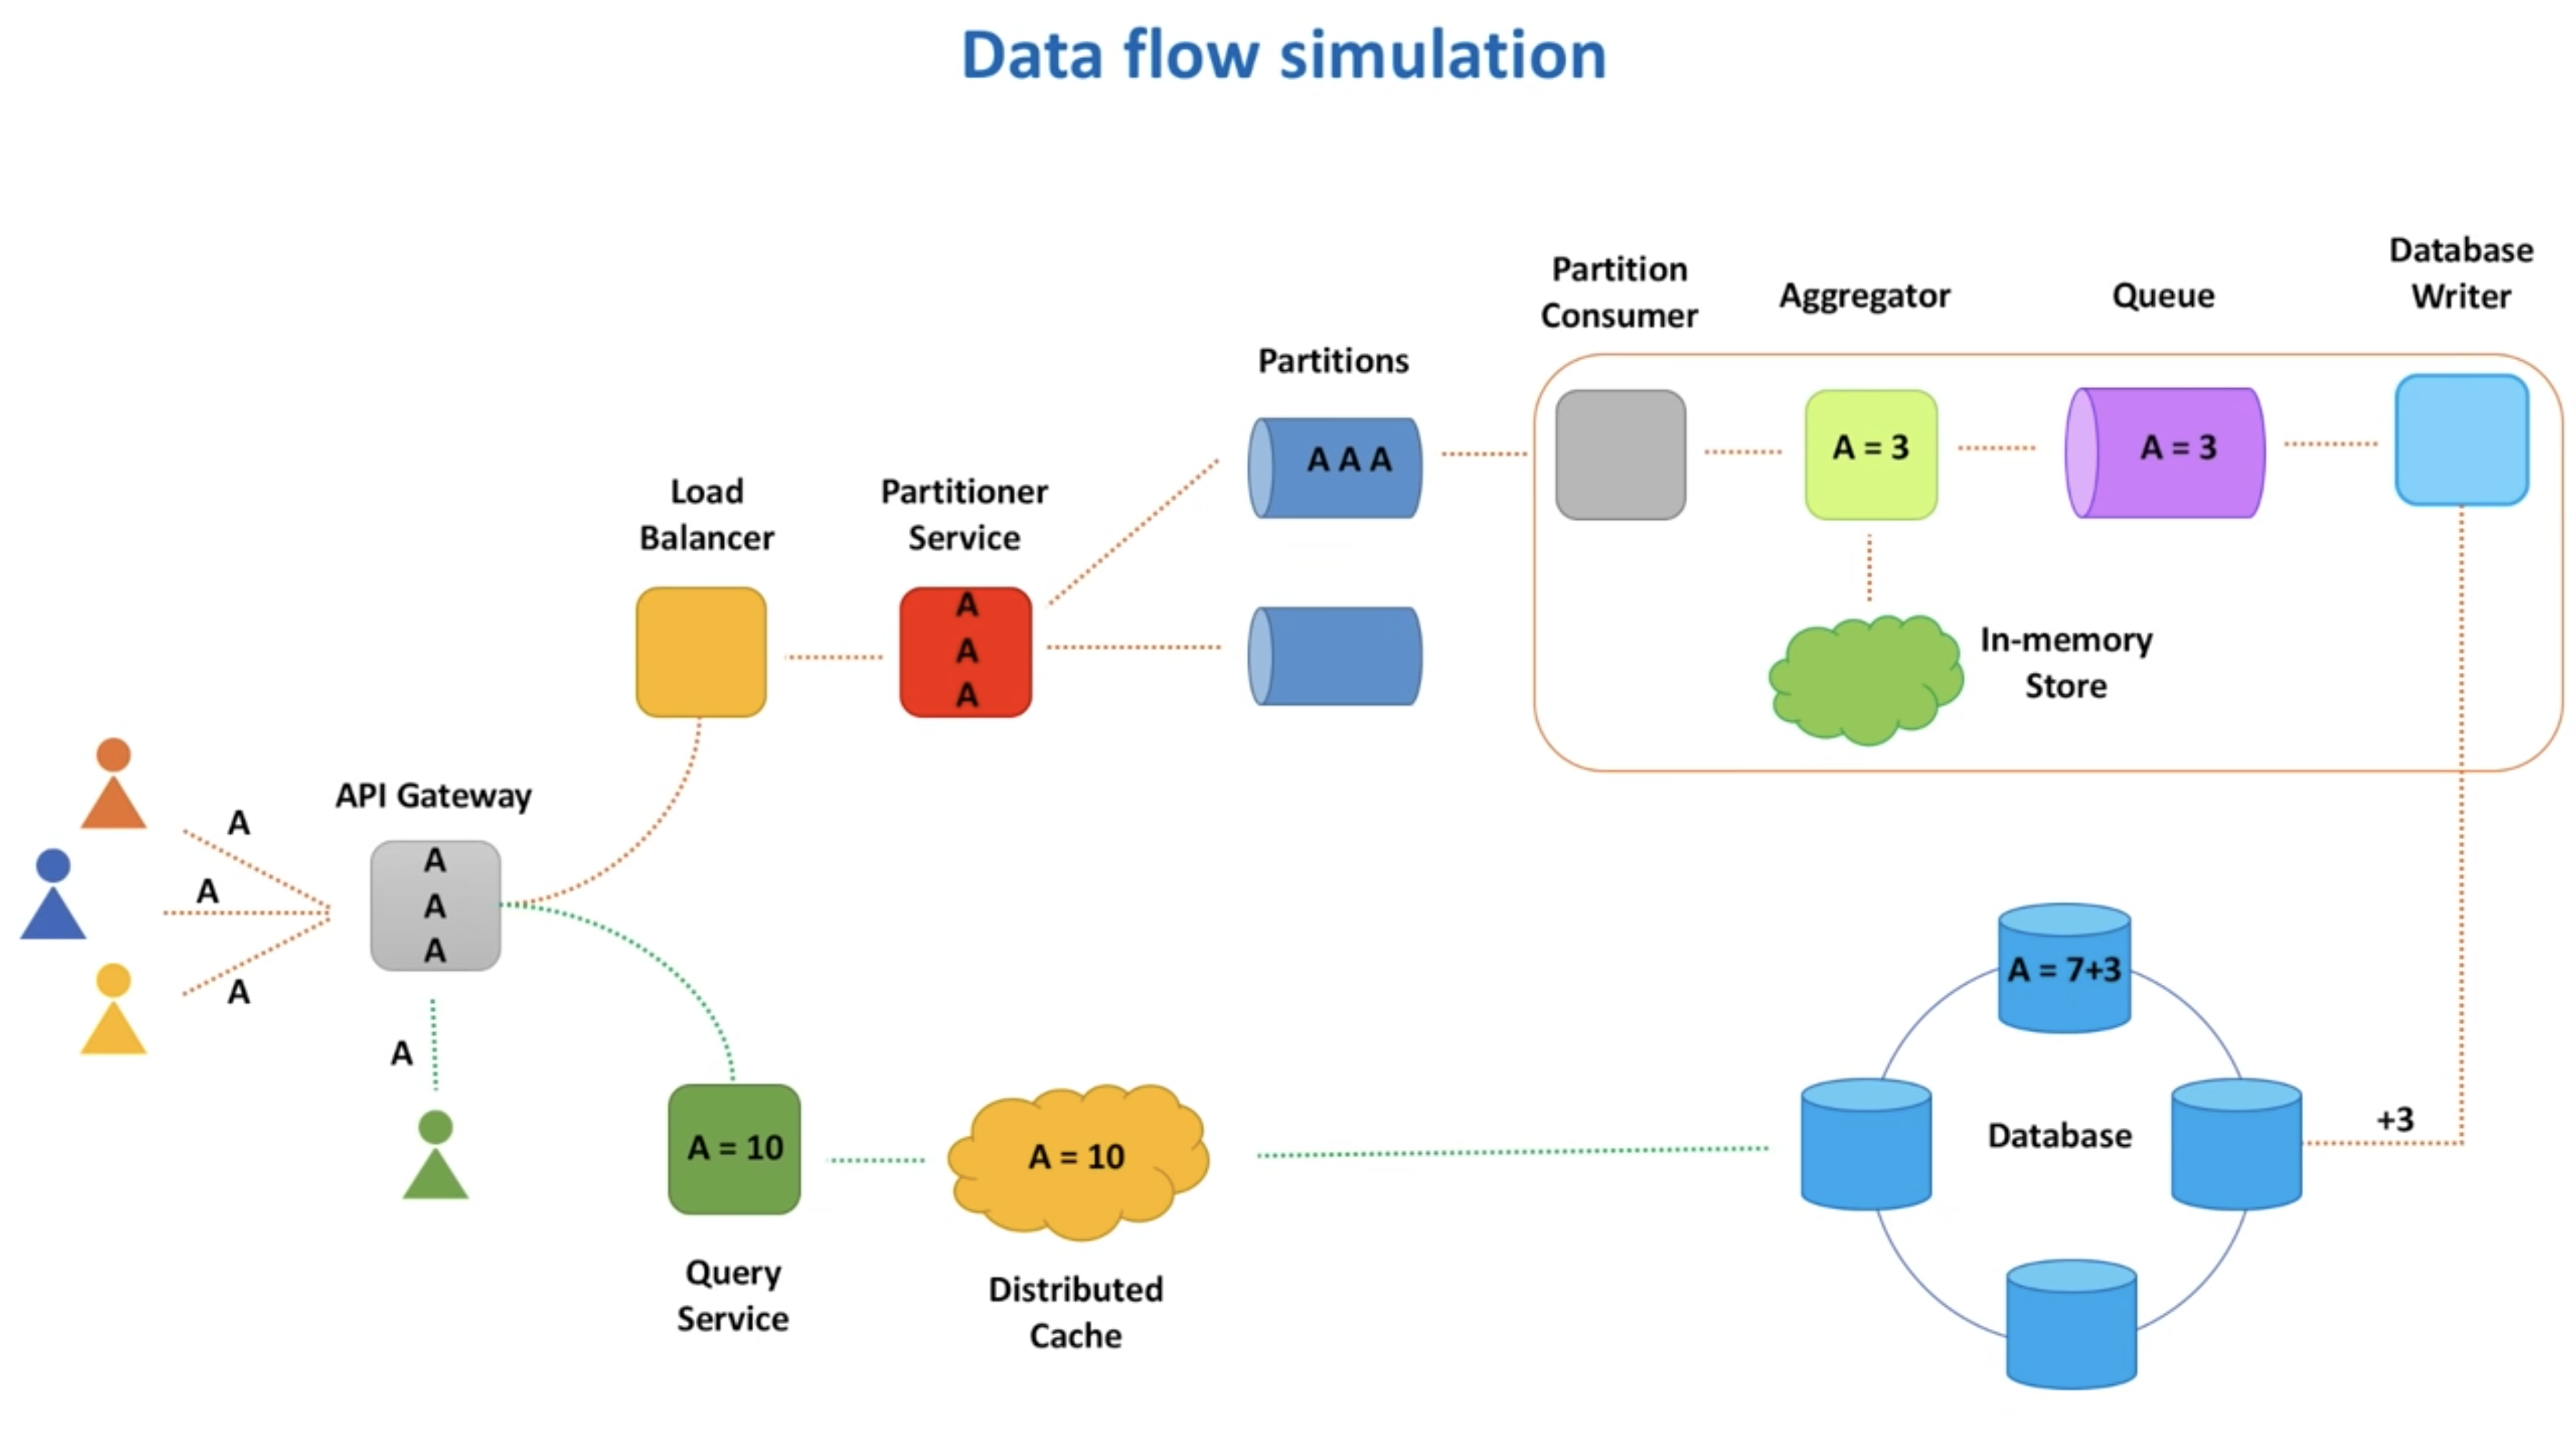
\includegraphics[scale=0.35, angle=90]{data-flow}

\end{document}

